%!TEX root = icse_seet16.tex
\section{Findings} % (fold)
\label{sec:Findings}

% Noel: Not sure why this is commented out, we need some preamble and this seems as good as any
We present the findings according to our research questions, and highlight the main themes that emerged alongside representative quotes from the interviews.
%Each participant quote will be identified depending on which course they were taking, as seen from Table \ref{table:interviews:students}. Before that, we provide some insights how GitHub was used in the courses in our case study.

\subsection{Student Benefits of Using GitHub for Software Engineering Courses}
Previous work~\cite{zagalsky2015emergence} has shown that GitHub introduces numerous and sometimes surprising advantages in the context of learning and teaching, however, it is important to consider how this is perceived by the students involved. Investigating the student perspective, our study reveals emerging themes on the student perceptions on the benefits of using GitHub in education.

%In this section, we discuss the benefits that emerged from the students' perspectives from the three main uses of GitHub in their courses: for schedule and material dissemination, for discussions, and for hosting their project work.  %Many of these benefits stem from GitHub being a tool commonly used in industry, as well as from the advantages that Git offers for managing individual and group work.

\textbf{Benefit: Gaining and Demonstrating Industry-Relevant Skills and Practices}\\
To succeed in modern software development, students need to be familiar with best practices (e.g., peer review, cross-team collaboration) and commonly used tools (e.g., continuous integration tools, distributed version control systems). Many of the interviewees [SE2, SE3, SE4, SE5, SE6, SE7, SE8, SE11, SE13, DS4] mentioned that using GitHub in their courses provided a good introduction to the tool and to relevant practices. \textit{``I think when you go and work in software development too, you should get used to [having] lots of eyes being all over your work; that's just the way it's gonna be, so it's practice before real life.''} [SE8]

% Students came into the course with varying degrees of experience with GitHub, as shown on table \ref{table:interviews:students}. Five interviewees had minimal or no experience using it, while others were very knowledgeable about the tool, either through their own uses, through group projects for other classes, or through co-op jobs. Many, at least those who attended the University of Victoria for the majority of their undergraduate studies, had some experience with Subversion, a different version control tool that is taught in a second-year course.

% Many of the interviewees mentioned that using GitHub in class provided a good introduction to the tool for them, even with just the basic use of GitHub to manage course activities such as material dissemination and discussion: \textit{``I think it's pretty good. I mean one thing is that because I'm using it in class, it's made me learn the tool \ldots and that's where the big takeaway is: that I've been able to transfer those skills, I've done some other projects just on my own time using GitHub.''} [SE2]

% For the most part, students who supported this theme believed that the use of GitHub for their courses and projects helped them experience a style of collaboration that they will encounter often in their careers. In comparison to the use of more traditional LMSes, one student noted why using GitHub might be advantageous for them: \textit{``Well, I like how it's the bonus of more practice of something you're gonna use in industry, whereas none of us are gonna use CourseSpaces or Connex when we're out on a co-op or out on a job.''} [SE3]

% Importantly, however, putting their projects on GitHub provides practice for real-life scenarios. SE8 describes why it was beneficial to have their work publicly available for both classmates and outsiders to see: \textit{``I think when you go and work in software development too, you should get used to [having] lots of eyes being all over your work; that's just the way it's gonna be, so it's practice before real life.''} [SE8]

% Beyond the benefit of using GitHub in programming projects, which is what it was designed for, the basic use of GitHub to manage course activities such as material dissemination and discussion was also beneficial to students as an introduction to the tool, with some caveats. \textit{``It's a good introduction to GitHub as a platform; it might not be a good introduction to Git as a tool. Because there's a lot of wizardry that you can do with Git that you'd never learn just doing what we did here \ldots but definitely a good start to get people using Git.''} [SE11]

Despite previous experience with the tool, using GitHub in their courses introduced some students to specific features that they were not necessarily aware of, features they believe are important to learn. \textit{``This is the first time I've actually used the issues portion of GitHub.''} [SE13] Even with the most basic use of GitHub in a course (material dissemination), students were able to reap the benefit of being exposed to a tool widely used in industry.

% Out of all the benefits described by students, the benefit of getting an introduction to GitHub and its features was talked about the most, as [SE2, SE3, SE4, SE5, SE6, SE7, SE8, SE11, SE13, CS4] specifically mentioned this benefit. The importance of this benefit is further emphasized by these students asserting their intention to continue using GitHub or to use GitHub even more after the course ends. This benefit was shared by students irrespective of their prior experience with GitHub. \\

% \textbf{Benefit: GitHub as a Portfolio} \\
% Many students believed that using GitHub to host their course projects will be beneficial to them in the future. These students described that hosting their code from other courses or from personal projects on their GitHub accounts benefited them in various ways. For example, SE5 organized their code on GitHub for easy access when helping friends: \textit{``I know that when you're trying to help somebody out, you can always just say `Check out my GitHub', I know I've done that with a few of my buddies \ldots and I don't have to search through my files, it's just on GitHub, and you look on there. It's a good organization tool.''}
%
Another important aspect of the use of GitHub is the current concept of mutual assessment~\cite{Singer2013} and the ability to use the tool as part of one's portfolio. Interviewees [SE5, SE6, SE7, SE8, SE11, SE13, DS3, DS4] mentioned the importance of publicly presenting their work on GitHub. It is not uncommon for employers nowadays to refer to GitHub for hiring purposes\footnote{\href{http://www.cnet.com/news/forget-linkedin-companies-turn-to-github-to-find-tech-talent}{http://www.cnet.com/news/forget-linkedin-companies-turn-to-github-to-find-tech-talent}}. In fact, some of the students we interviewed had already been contacted by potential employers who wanted to view their GitHub accounts: \textit{``I think all three companies that I applied to this semester wanted me to link to my GitHub. So I was really lucky that I had [a class] project on there. And I think when this [course's] project is done too, it'll also be really nice to have up there, after we clean it up.''} [SE6]

% CS2 also shared that interviewers inspected their code during an interview, highlighting the importance of having functional code in one's GitHub account: \textit{``These days I see that employers also want to see your GitHub page. While I was giving an interview for my coop, he did actually go into my GitHub profile and try to compile some of my code, so they do want you to have some online presence on GitHub.''}

%\textit{``Well I believe it's good for future employers. I remember I put directly on my resume saying you can check out the work I've done on GH. I included the link right on there and every person I handed my resume to were just like \'hey, fantastic!\' \ldots it's a good way to get your skillset out there.''} [SE5]

%The ability for students to use GitHub as a portfolio where they can show off their projects to potential employers was, for many, an important benefit of using the tool. There were students who were introduced to GitHub as part of their course, but knew the importance of having work on GitHub. This benefit motivated some students to continue putting their work on GitHub.
% The benefit of using GitHub as a portfolio was shared by [SE5, SE6, SE7, SE8, SE11, SE13, CS3, CS4]. \\

\textbf{Benefit: Enabling Cross-Team Collaboration and Contributions}\\
%In these courses, projects were open and visible to other students, creating opportunities for student contribution, a workflow that GitHub encourages. This was demonstrated by a student's group getting feedback from and providing feedback to others: \textit{``For instance, one [issue] was our script wasn't taking in command line arguments if there were spaces in them properly. And then someone [gave us a suggestion that we used]. And then to be able to see what other people are having problems with and give suggestions.''} [SE3]
Requiring students to host their course projects openly on GitHub and the heavy reliance on GitHub in the course resulted in students looking at and contributing to the work of others. Students provided feedback and received suggestions from others [SE2, SE3, SE5, SE7, SE10, SE11, SE12, SE13]. And while some lab assignments required students to look at the work of other students, many students reported that they would often peruse other projects outside of the requirements. In a few cases, students utilized code that other groups built, and as a result, helped them discover and fix issues in the original code. \textit{``I believe that one other group decided for project 2 to use [our project 1] and they made a couple of Pull Requests I think.''} [SE10]

By facilitating student contributions and cross-team collaboration, the use of GitHub enabled a participatory culture~\cite{jenkins2009confronting} where students openly created and remixed content and felt their contributions mattered. As a result, GitHub encouraged peer review practices among students: \textit{``I thought [peer reviews] was the best way to learn actually \ldots It forced you to put yourself in a position where you have to defend what you did, which I think is good for quality because you have to actually care.''} [SE11] The use of GitHub also provided collaborators in group projects an easy way to track and keep up with each other's work: \textit{``You can see exactly what the other person has contributed, and you can look it up again a month later \ldots then it's a good way to keep accountable. And it's good for yourself too, because you know they can see your work, so you wanna make sure that it's top notch and easily readable.''} [SE5]

%The ability to open up student work to anyone simplifies the peer review process, particularly with the `social coding' emphasis of GitHub where others can make inline comments or corrections themselves.

% Helping other projects, either through discussion or through collaborating on the code, offered students new ways to participate that are unique to GitHub and similar types of systems. Students effectively collaborated with each other with the aim of producing better work, as was noted by [SE2, SE3, SE5, SE7, SE10, SE11, SE12, SE13]. \\

%\textbf{Benefit: Keeping Each Other Accountable} \\
%One benefit that stemmed from GitHub's transparency features was the ability to see a history of commits to a project. This was cited by some students who used GitHub to manage their group projects---they could easily see if and when their partners submitted work. Their repositories kept an account of when each change was made, which provided collaborators an easy way to track the work being done on the project. This helped the students to keep up with each other's work: \textit{``You can see exactly what the other person has contributed, and you can look it up again a month later \ldots then it's a good way to keep accountable. And it's good for yourself too, because you know they can see your work, so you wanna make sure that it's top notch and easily readable.''} [SE5]

% Moreover, the students knew exactly how much work each member of their group contributed to the project and this helped the student keep themselves and each other accountable: \textit{``We decided to switch to pull requests instead of just committing straight to master, because \ldots for a couple of reasons, first of all, if there's something majorly wrong with it, everyone can see it, right? And the second thing is, everyone sees it, so if people have to work on [the same code], in the future, which we all did, then they know exactly what just went in, so that next time they come to the code and pull it, they're not like `where did this all come from?'\,''} [SE9]

% This is a useful feature to have when working in group work as it allows for awareness between group members. By using GitHub for their group projects, students were able to take advantage of the collaborative features that GitHub offers to improve their processes or their product. This benefit was described by [SE5, SE9, SE11]. \\
%%%http://www.cs.usask.ca/faculty/gutwin/866/2010-T2/readings/p72-gutwin.pdf

\textbf{Benefit: Encouraging Student Contributions to Course Content} \\
One of the benefits that GitHub offers over traditional Learning Management Systems is the ability for students to suggest corrections and make changes to course materials via Pull Requests (PRs). This is a simple change mechanism that provides students with a degree of autonomy, but that instructors can easily accept, reject, or request resubmission.

Throughout the two courses in this case study, three PRs were submitted to make corrections to the course materials or to add links to new materials. These PRs were submitted during the first month of each course and by a single student (SE1) that had previous experience with GitHub (the student was registered in both courses). SE1 commented : \textit{``I like being able to fix the mistakes that [the course instructor] might make, like with a bad link or something, by making a PR\ldots because it makes me feel a little more involved.''}

%However, the lack of timely PR acceptance was not the only issue at play. It is possible that the lack of contribution to the course materials was also due to GitHub's \emph{diff} feature and its lack of support for non-plain text files. Some of the course materials used during the case study were in PDF or PowerPoint form, which students [SE12, SE13] indicated made the process of suggesting changes \textit{``inconvenient''}, a limitation also mentioned by educators~\cite{zagalsky2015emergence}.

It is interesting to note that this style of student contribution didn't continue. A few of the interviewees [SE1, DS2, course instructor] reported that the PRs were not merged \textit{``quickly enough''}---the students expected an immediate response (due to a deadline), but the instructor did not merge them for a day or two. Nonetheless, students [SE1, SE3, SE5, SE6, SE10, SE13, DS2, DS4] felt that contributing to the class materials could have been a useful exercise had they taken advantage of it or had the possibility to do so more advertised.%\todo[inline]{CP:you should mention the lack of advertising...I think the last time I saw it was way up in methodology (and it seemed out of place up there)}

% Another student described how this hindered more participation of this kind: \textit{``Because we did not have the access. If we had the access, then I think people would have collaborated''} [CS2]

% Although SE6 did not contribute in this manner, they saw the potential advantages of using pull requests as follows: \textit{``I think everybody's had experience with mistakes in the course material. \ldots The alternative is just emailing the prof and asking them to change something \ldots this is always there, and they can always check it to see if there's something. This way someone can actually make the change, all they'd have to do is accept it.''} %SE6 discussed the convenience this feature offers to instructors, as changes are listed on a separate page in the GitHub repository and can be accepted with one click. Of the three PRs submitted to the courses, two other students participated by either trying to accept the PR (and failing), or adding a `+1' to the PR's comments, supporting its acceptance.

% However, this method of contributing to the course is limited because of the types of files GitHub supports.  \\ %Nevertheless, the following students agreed that being able to contribute to course materials via GitHub is a benefit: [SE1, SE3, SE5, SE6, SE10, SE13, CS2, CS4]. \\

\textbf{Benefit: Breaking Down the Walled Garden} \\
Work hosted on GitHub is often publicly available for others to see and contribute to, allowing interactions with external entities (i.e., practitioners and experts). Our study revealed a case where a student [SE1] invited community engagement. The student was an active member in the Rust programming language community and advertised their course work to that community. As a result, members of the community tried to help with the project in multiple ways: \textit{``So here I have people involved in the discussion. These are just people in the community I've been talking to about how to do different things, and they've been giving me suggestions. And that's really cool because I actually have some community involvement in my course project.''} [SE1] And while considered an outlier, this example illustrates the ease of supporting external interactions and the potential of tapping into new sources of knowledge, effectively breaking the \textit{``walled garden''} imposed by traditional LMSes~\cite{mott2010envisioning}.

% SE1 was the only student interviewed who used the public nature of the course projects to solicit outside contributions. However, the exposure to GitHub gave students opportunities to discover work outside of the course and to use other repositories to aid their projects. When prompted, most interviewees mentioned that they sought out public repositories either to pull their code and use it, or to find inspiration for their own projects. One student recalled an experience where their group looked at an open-source library: \textit{``We just looked at how Gitstats, [an open-source library] did it, and then wrote our own thing into our project \ldots I think that more than anything is the biggest reason why Git should be used for education, because it takes, I think, until you start being forced to do it \ldots to actually go and look at other people's code, and I think looking at other people's code is the most important thing.''} [SE6]

% Speculatively, however, this likely would have happened regardless of whether or not GitHub was pushed by the instructor as students tended to seek out other code and libraries for their projects: \textit{``And in industry, the first thing you do is check Stack Overflow, look for someone else who has done the same thing and jack their code.''} [SE7] [SE1, SE2, SE3, SE4, SE6, SE7, SE10, SE12, SE13, CS2, CS5] mentioned looking at outside work and public repositories for their projects.

\textbf{Benefit: Version Controlled Assignments}\\
% Using version control for their assignments and projects benefited the students in multiple ways. The ability to revert to previous states of the code was useful: \textit{``You're working on a project, and you make a change that breaks everything. Well you can just go back to a different commit, one that works. Boom, fixed, try again.''} [SE11]
%
Some students [SE8, DS3] noted the possibility of using GitHub's history and version control mechanism for providing continuous and constructive feedback. \textit{``You'd see all the mistakes [the student] made getting there, too, which is just as important to learning as the finished product.''} [DS3] While this feature was not utilized in these courses, students saw how the feature provides one with the ability to examine the final product, as well as the process used to get there.
% SE8 described a the potential of using GitHub for grading, where instructors could use the student's repositories as submissions as opposed to the traditional way of submitting through an LMS: sending the code only when finished. SE8 said that this way of submission would be \textit{``so much more useful \ldots You could see everybody's contributions, you could comment on them too \ldots Unless you're doing a live code demo with a TA or any instructor, you're not getting any real feedback [with the traditional submission system] \ldots You have no idea where you lost the marks or where you went wrong.''}

\subsection{The Challenges Students Face When Using GitHub for Software Engineering Courses}
Our case study provided a glimpse into the challenges students may face when using GitHub for software engineering courses.
%This section outlines the challenges the students described relating to GitHub use in courses. Some of these challenges were related to tool literacy, where more knowledge of the tool and more experience using it in an educational context could have mitigated the challenges. Yet they are worth mentioning as potential challenges that students might encounter. \\

% Noel: I renamed this quickly from 'Privacy is All-or-Nothing', I think it better describes the point. That said, not sure about the name!
\textbf{Challenge: The Perils of Public Projects}\\
%While publicly sharing student projects on GitHub publicly provided several benefits, others acknowledged that it may not be appropriate for other class environments. SE4 describes this dilemma: \textit{``So [using GitHub for your work has] got benefits and drawbacks: benefits being that other people can access your data, drawbacks being that other people can access your data.''}
Having the course materials and students' work open to the outside world can be a double-edged sword. On one hand, it allows students to benefit from interactions with people external to the project, as previously mentioned. On the other hand, students had concerns that should not be ignored.

The students we interviewed didn't mind that the class repository and their project work was publicly shared on GitHub. However, several students [SE1, SE4, SE5, SE6, SE7, SE10, SE13, DS3, DS6] recognized the potential problems that might surface from publishing their work publicly. They mentioned two possible issues: 1) their school work may not be of interest to the public, and 2) their work may not be at a level they feel comfortable sharing, especially when colleagues and potential employers may see it.
\textit{``It would actually be nice if [our projects] were separate or private somehow so I wouldn't have to go through everything and sanitize all the stuff I've submitted, because for as much as you'd want to think you're putting 100\% into it, you're not really.''} [SE6]

%For example, CS3 noted that although it can be advantageous to host code publicly so that employers are able to see their projects, the employer may not always agree: \textit{``I think it comes back to what do you want to show your employers? When your employer looks at your work, will they understand that work I submitted in Git was when I didn't yet understand what I was doing, I was still learning? \ldots If I could make the assumption that an employer would understand that, I would have no problem with it being public. That said, I can't make that assumption. I have to assume that everything they look at they're judging in the harshest light possible. So I try to show only things that are of quality that I'm proud of. And that's unfortunately not a lot of the classwork until I'm done with it \ldots The final product I'm happy to show, but all those steps getting there, they're often filled with pitfalls and horrible programming and badly factored code.''} As such, courses mandating the use of Git and GitHub to publicly host student work could be problematic for students if employers are looking at work-in-progress in a negative light.

%not everything is 100% effort
% SE6 acknowledged that sometimes, students rush through their work, and therefore, they might not want that work to be publicly available: \textit{``You know it would actually be nice if they were separate or private somehow so I wouldn't have to go through everything and sanitize all the stuff I've submitted, because you know, for as much as you'd want to think you're putting 100\% into it, you're not really, you know, writing some great work of art or careful analysis, so private would be nicer. For things like that.''}

%not everything is of interest to public
% As well, SE1 felt that some of the work in the course repository wouldn't even be of interest to the public or to potential employers, and as such, they saw no need for the repository to be public: \textit{``I'd rather have [our comments] be private. But only because there's not a whole lot of participation, so I don't feel they're of interest to someone publicly.''}

% \emph{Discrepancy:} However, others saw no issue and even preferred all their work be in the public space. \textit{``Personally I don't have a problem with it being public. I would like to have a good online activity of myself on GitHub, so that's not really an issue. I'm not really concerned if someone is going to read my blog or not.''} [CS2]

Not surprisingly, students found a workaround to some of these privacy issues---students do not have to attach their full names to their work on GitHub, or they can even use a separate GitHub account. \textit{``You can decide that on your own, depending on if you use your main git account or just make a separate git account for your class.''} [SE3] Our case study revealed a student that created a new GitHub account solely for their contributions in class. However, this student refused to be interviewed.
It is important to note that not all the interviewees shared this concern, and a few [SE5, DS2, DS5] didn't see any privacy concerns with sharing their work publicly.

% In summary, although students enjoyed the benefits that came with making their work publicly available, many students also acknowledged that these benefits are accompanied by a number of caveats. Importantly, some students described the lack of a middle ground as a limitation, where in the context of this course, students had to host their work publicly. This challenge may be mitigated by the instructor giving the students the option of creating a new GitHub user account for work done in their courses, as suggested by SE3 above. This challenge was shared by [SE1, SE4, SE5, SE6, SE7, SE10, SE13, CS3, CS6], while [SE3, SE5, CS2, CS5] disagreed on these issues. \\

\textbf{Challenge: Unfamiliarity with Git and GitHub}\\
% For example, SE9 believed that students who were less experienced with the tool could not take advantage of its benefits, such as the ability to make pull requests on the course materials. SE9 believed that if the instructor did not set a precedent for that behavior, it may not be used: \textit{``I think you just have to advertise it so that the students know [to] use this as a communication tool. And then layout or give some examples on how it could be used.''}
When asked about challenges, students mentioned how an unfamiliarity with Git and GitHub caused difficulties and missed opportunities in taking advantage of existing features (e.g., Pull Requests, GitHub issues) [SE1, SE2, SE3, SE4, SE5, SE6, SE9, SE11, SE12, SE13, DS1, DS3, DS5].

%Another issue that many students [SE1, SE2, SE3, SE4, SE5, SE6, SE9, SE11, SE12, SE13, CS1, CS3, CS5] described related to education and training is that there were varying degrees of experience with and knowledge of GitHub and its features, which presented difficulties with the use of GitHub in these courses.
Furthermore, the course instructor was inexperienced with using GitHub, which made it difficult to educate the students on its features and caused frustration for some of the interviewees. Students [SE6, DS1] suggested that an introduction lecture dedicated to learning how to use GitHub at the beginning of the course would have been helpful. Others [SE1, SE2, SE3] proposed that this challenge could have been alleviated by a greater focus on version control and version control tools earlier in the curriculum.
%In fact, most students who were asked mentioned that the course could have benefited from more education on Git, GitHub, and what they can do with it. Students said that they could have hosted a lecture or a lab dedicated to learning the tool, perhaps at the beginning of the course or as an extra session. \textit{``I think it would've been good to do some demo \ldots cause I think [the instructor] talked too much about theory in class and there's no actual coding or no actual demoing.''} [DS1]

% SE2 acknowledged the potential difficulties in hosting such a session: \textit{``On the other hand, when someone teaches it to you, it often doesn't make sense until you actually do it yourself. Cause you'd actually have to go through the struggles of actually doing a commit and pressing all the buttons, so I don't really know how much could be done in that regard.''}

% Students also asserted that the University of Victoria needs to further emphasize teaching version control systems such as GitHub at the undergraduate level. As it stands, there is one required course that teaches version control systems and how to use them, utilizing Subversion and touching on Git. Some students, however, felt that one course was not enough, particularly when Subversion is not very popular anymore: \textit{``I think in [SENG265], we did SVN, which is a good introduction to the idea. But I don't think it's widely used anymore.''} [SE3]

% Three of the interviewees [SE1, SE6, and CS3] believed that students should get an account quickly after their first introductory Computer Science courses. \textit{``If I was teaching someone how to code, as soon as they start working on code that was bigger than 100 lines, I would teach them how to use version control.''} [SE1]

%This is an issue of tool literacy and an instructor who was experienced in using GitHub might have been able to better educate their students on GitHub and the features they intended to use.
%asserted that this issue could have been alleviated by a greater focus on version control, DVCSes and what students can do with these tools earlier in a curriculum. As it stands, students were not able to properly utilize some of the benefits of using GitHub due to inexperience and unfamiliarity. %This was discussed by [SE1, SE2, SE3, SE4, SE5, SE6, SE9, SE11, SE12, SE13, CS1, CS3, CS5]. \\

\textbf{Challenge: Notification Overload} \\
%Although few students brought up this issue, how GitHub handles notifications from the repository nevertheless emerged as a challenge.
Another challenge lies in how GitHub handles notifications and one's level of familiarity with the possible options. GitHub's mechanism for managing notifications is the `watch' functionality, where for every repository there are three options:
\begin{itemize}
    \item \textbf{Not watching}: The user receives notifications only when participating or when their username is mentioned.
    \item \textbf{Watching}: The user receives notifications on all conversations and activities (e.g., commits, PRs, comments on issues).
    \item \textbf{Ignoring}: The user does not receive any notifications.
\end{itemize}
Each user can also control whether the notifications are shown in the tool itself, sent by email, or both.

%1) to get a notification and an email only when the user is mentioned in issues or commits, and in discussions the user has commented on; or 2) to get a notification and an email when anything at all happens in the main branch (master), when someone comments on issues, commits, or pull requests, and when someone makes or accepts a pull request. %The `Watch' feature comes with some drawbacks, not the least of which was how a student's lack of familiarity with the feature prevented them from using it: \textit{``I didn't like that [repository] at all, because I didn't get notified when [the instructor] adds stuff to there, so I don't really know what's going on without remembering to check it on GitHub. ''} [SE9] This student did hear about the `watch' solution, but thought that it \textit{``would be a good solution, but it might be overkill. For like a spelling change.''} [SE9]

Unless students were `watching' the repository, they did not receive email notifications for any activities except when they were specifically mentioned. However, when the students did `watch' the repository, they received an influx of notifications for every user comment, which became overwhelming. SE10 shared that they were engaged less in the activities of others because of the noise from notifications: \textit{``It sent me a million emails, both of [the tools] actually. I should have just turned that off, but I was worried about missing something. Because every time someone would post, you would get another email \ldots I actually did not read anyone else's feedback because it was just so many emails, to be totally honest.''} [SE10]

% As such, the `Watch' feature was problematic for courses like the ones studied, where every single comment would trigger a notification and an email, causing an overload of notifications. [SE7, SE9, SE10, SE11] shared this issue.

\textbf{Challenge: GitHub is Not Designed for Education}\\
Students [SE2, SE5, SE6, SE7, SE9, SE11, SE12, SE13, CS4] described one drawback from using GitHub for education: GitHub is simply not built for it. Those that mentioned this particular drawback acknowledged that although there may be workarounds for many of the tasks needed, GitHub certainly struggles to meet some basic educational needs, such as gradebooks and a formal assignment submission feature. This was one reason why the course instructor for this study decided to use a customized version of Moodle in conjunction with GitHub---to ensure privacy with matters such as grades or to make announcements, something that would be too cumbersome to do in GitHub.

This issue potentially hinders some of the benefits listed above. For example, it is more difficult to contribute to course content because GitHub's \emph{diffs} feature does not support file types commonly used in education (such as PDFs and PowerPoint presentations). \textit{``I think one drawback of GitHub is that you cannot actually see the diff [of] commonly used files such as PPTs or PDFs, so you can't really use it for correcting professor's slides, or PDFs.''} [SE12] The pull request process then requires an extra step, which some students felt would discourage them from using this feature. \textit{``I think for readme files, it's a lot easier to edit, cause you can edit directly in GitHub. But for other files, you'll probably have to change and make a branch and then commit it and then send a PR, it might actually be more work.''} [SE13]

\subsection{Recommendations for Software Engineering Instructors}
% Given that the use of GitHub in these courses was relatively basic, many students, particularly those who were experienced with using GitHub for collaboration purposes, had ideas on how GitHub could be further utilized to be more beneficial for both themselves and for their instructors. Many students discussed recommendations such as which classes GitHub could best serve and the need to utilize additional GitHub features. This section outlines those responses, highlighting the suggestions students gave about the workflow for using GitHub in a course. \\
%In this section, we discuss recommendations for educators wishing to use GitHub to support their teaching. We extract relevant insights from the students and the teaching team regarding how GitHub can best serve courses in the future.

%\footnote{\url{alexeyza.com/blog/2015/09/10/embracing-participatory-culture-in-education}}
A main challenge educators face is the lack of a shared knowledge base~\cite{zagalsky2015emergence} on how to use GitHub to support learning and teaching. Some educators have shared their experiences and recommendations with others, either as personal blog posts or as part of a discussion\footnote{\url{https://github.com/education/teachers/issues}}. Additionally, GitHub provides basic guidelines\footnote{\url{https://education.github.com/guide}} for setting up an organization for a class, and has developed a command-line tool\footnote{\url{https://classroom.github.com}} to help set up a class repository. Contributing to these resources helps build a common knowledge base for instructors to share with and learn from. As a main contribution of this study, we illustrate the recommendations to instructors and educational tool designers below.
%Their classroom guide is useful for those looking for a step-by-step process, where they recommend applying for an organization for a course and assigning a private repository for each assignment for each student. Likewise, it can also be helpful to use the available resources: use GitHub support, look for other instructor experiences for guidance, or discuss experiences in a blog or in spaces dedicated to the topic\footnote{\url{https://github.com/education/teachers/issues}}. Contributing to these resources can serve towards building a common knowledge base for instructors to share to and learn from. Moreover, GitHub recently released a tool that automates many of the tasks educators need to set up on GitHub \footnote{\url{https://classroom.github.com}}. \\

\textbf{Recommendation: Promote the Desired Workflow}\\
As discussed earlier, students raised concerns regarding the public nature of the work they host on GitHub. As way to alleviate this concern, educators can promote the option of using pseudonyms to be used only for the course.
Students who were more experienced with GitHub also mentioned that some of GitHub's collaborative features should have been further utilized to provide additional benefits [SE3, SE5, SE6, SE7, SE11, CS2, CS3, CS4, CS6]. They felt there was little reason to use GitHub for a course if it was only used for material dissemination. They also noted that while there's potential, the unidirectional nature of the work being performed meant that potential benefits were not realized. \textit{``If there was a way to collaborate on the material, that would be useful \ldots But in this class, every one of our labs so far has been demo to the lab TA, so nothing's going back to GitHub \ldots Maybe if we were submitting things to it, maybe that would be helpful. I can see how it could be useful, it's just that in our usage it's not really adding anything to the experience.''} [DS3]

%For example, as mentioned above, only three pull requests were made throughout the semester.
%DS3 was outspoken on why using GitHub for this course was somewhat unnecessary: \textit{``I don't see any benefit that GitHub has offered that we wouldn't have had in [Moodle]. All it appears to me is it's a place where it's a file repo \ldots and we already have that.''} They also noted that while there's potential, the unidirectional nature of the work being done meant that the potential benefits were not realized. \textit{``If there was a way to collaborate on the material, that would be useful \ldots But in this class, every one of our labs so far has been demo to the lab TA, so nothing's going back to GitHub \ldots Maybe if we were submitting things to it, maybe that would be helpful. I can see how it could be useful, it's just that in our usage it's not really adding anything to the experience.''} [DS3] A number of students [SE3, SE5, SE6, SE7, SE11, CS2, CS3, CS4, CS6] expressed concerns that GitHub was not being used to its full potential in their course.

% SE7 echoed these sentiments: \textit{``I think that you can accomplish the same thing with a simple HTML website, honestly \ldots It's not using a lot of the features of Git, like looking at changes, commits, pull requests. The issues were kinda cool for the lab, and, again, you can accomplish that with any sort of forum, I would think \ldots We're not actually delivering code to the professor, so maybe it doesn't make a ton of sense [to be using GitHub].''}

% As such, many students believed that GitHub was not being used to its full potential in their courses. The underlying suggestion was to consider which features of GitHub the instructor would like to use, such as pull requests or grading via commits, and use those features thoroughly and consistently. As it stands, some of the benefits they described to using such a system were only possibilities. An example, which will be highlighted later in Section 5.8, was reported from a student in the CS course, where even the issues were not used for discussion during labs: \textit{``So basically we had to show it to our TA that we have done [the lab], and [the TA] used to mark it in a piece of paper. So putting [our responses in the issues] was not really necessary?''} [CS2]

Consequently, students [SE3, SE5, SE6, SE7, SE11, CS2, CS3, CS4, CS6] stressed the importance of defining a workflow when using GitHub in a course and then advertising the desired workflow to the class. For example, promoting the use of Pull Requests as a way to suggest corrections to course materials, or encouraging student-to-student feedback and contributions. \textit{``I think it would've needed to have been advertised more that [the instructor] was looking for input on things, and if [the instructor] said that, maybe more people would have [contributed] to maybe propose extensions for assignments or something.''} [SE7] However, merely promoting the workflow is not enough. GitHub is a powerful framework, but it is up to the instructor to consider which features they would like to use and how (e.g., PRs for assignment submission), and use those features thoroughly and consistently (e.g., merging PRs more quickly).

% \textbf{Recommendation: Define and Advertise a Workflow} \\
% Students acknowledged that GitHub was not being used to its full potential and that there was confusion surrounding the use of two tools (GitHub and CourseSpaces). CourseSpaces was used to fill some of the gaps in education support offered by GitHub, such as private forums and a gradebook. However, students tended to be displeased with this decision. \textit{``One thing I really don't like is that we have both systems set up, and so sometimes the announcements are in GitHub, and some of the times, they're in CourseSpaces, and that can get kind of confusing, like did [the instructor] post an assignment here or there?''} [SE2]

% This was an almost unanimous issue between the students interviewed, with only a few stating that they did not mind either way. Most mentioned that they would have preferred the use of just one tool, even if everything was public in GitHub. As a result, many students suggested that it would have been important to define a workflow for using this tool in a course in order to gain the benefits described earlier in the chapter. This workflow could include aforementioned activities such as utilizing pull requests or using just one tool instead of two. In the case of pull requests, for example, students advocated that the instructor should be advertising their use, thereby defining to the students that contributing to the material would be part of the course workflow: \textit{``I think [the idea is] good, but I think it would've needed to have been advertised more that [the instructor] was looking for input on things, and if [the instructor] said that, maybe more people would have [contributed] to maybe propose extensions for assignments or something.''} [SE7]

% One student mentioned that although GitHub does not do everything needed in a course, defining a workflow will cover up many of those weaknesses: \textit{``Even if there are no enhancements on GitHub, but if you define a proper workflow for using it, then it can be quite successful, because even the present Learning Management Systems are not perfect right?''} [CS2]

% While most students did not have suggestions as to what workflow to use, they acknowledged the importance of defining it and teaching it to the students early on in the course. SE6 wanted to \textit{``enforce more actual Git and GitHub features in the way that we interact with the course material, and enforce GitHub use for actual projects. In a way that everybody had sort of a base level of understanding. So maybe at the beginning of the course \ldots there should definitely be a time when you learn Git.''}

% In summary, many of the students interviewed were frustrated by the lack of a clearly defined workflow, and believed that the course would have been improved greatly if a workflow had been created and advertised in the beginning. This recommendation emerged from interviews with [SE1, SE2, SE3, SE4, SE5, SE7, SE9, SE11, SE12, SE13, CS2, CS3, CS4, CS5].

%\textbf{Recommendation: Use GitHub in More Open-Ended Courses} \\
\textbf{Recommendation: Familiarize Yourself with GitHub}\\
Several students questioned the possibility of using the same workflow for all courses, however, GitHub actually provides mechanisms to determine the level of privacy depending on the workflow used. For example, if educators wish to have the course material and assignments open only to students, they can create an organization on GitHub just for the course.

%While most students interviewed did not mind their work and comments being in the public space, there were concerns regarding how this way of working could apply to different types of courses, particularly courses in which students are afforded less freedom in the nature of their work. Students [SE2, SE5, SE6, SE7, SE13] suggested that a course similar to the two cases studied, where the work is very open-ended and could exist in a public space, is where using a tool like GitHub would benefit students the most: \textit{``I would say this class is specifically different because we had so much flexibility over what we were doing. It's not like in our Operating Systems class, [where] we make a shell that does this, this, and this. This was way more open ended, everyone's doing something different, so even if you could see what everyone else is doing, no one could've helped us.''} [SE7] In using GitHub for courses with more open-ended assignments, the benefits we highlighted earlier, such as eliminating the walled garden, allowing students to contribute to each other's work, and allowing students to build an online profile, can be realized. Moreover, the educator can introduce an element of peer review that students may benefit from \cite{sondergaard2012collaborative}

On the other hand, in courses where student plagiarism is a concern, educators can use private repositories while still taking advantage of the other benefits that GitHub offers. In order to set up an appropriate workflow, educators can either create private repositories for their students or ask the students to do so themselves. This workflow would require students to submit assignments with the use of PRs.
%\footnote{\url{https://education.github.com/guide/private_repos}}

\textbf{Recommendation: Use Supported Formats}\\
In order to simplify the contribution process, we also recommend the use of plain text file formats (e.g., Markdown, iPython documents) in order to take advantage of the \textit{diff} and line commenting functionalities.

%Because all work is version controlled, an educator can keep vigilant for possible instances of plagiarism, as Kelleher~\cite{kelleher2014employing} does. The professor who taught the courses in this case study agreed: \textit{``There was a difference between what we saw in terms of the code repo and how students were participating in their own repos and some of the things that they were handing in. \ldots I think for us, these subtleties are important.''}

%%% start of validation survey %%%

\subsection{Validation Survey}
\begin{figure*}[t]
\centering
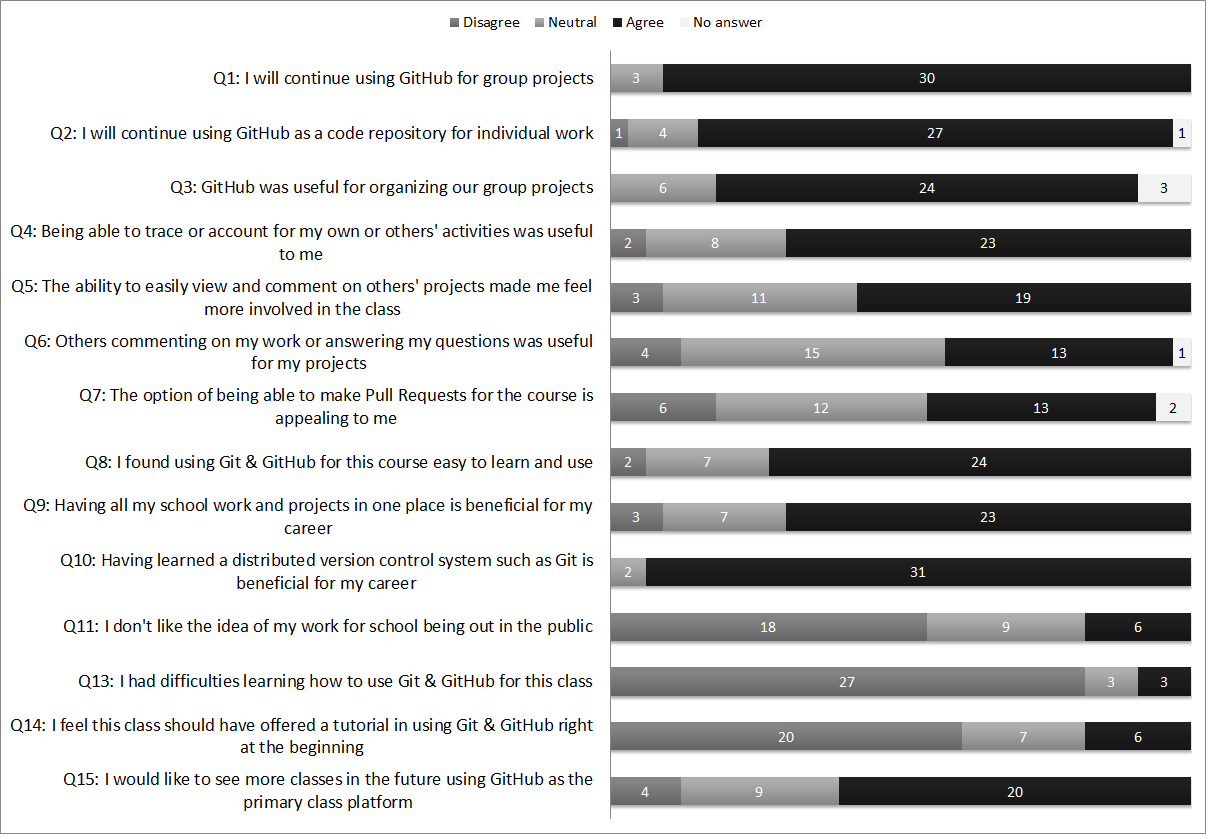
\includegraphics[width=0.75\textwidth]{surveychart}
\vspace{-4pt}
\caption{Aggregate of responses to validation survey questions}
\vspace{-12pt}
\end{figure*}

To validate the themes that emerged from the interviews, we sent a survey to all of the students in both courses at the end of the term (during the last week of the course). 33 students (18/34 DS and 15/29 SE) responded to the survey, giving us a response rate of 53\%.  The survey consisted of a set of Likert scale-style questions that were designed and pilot tested to confirm or refute our findings concerning the benefits and challenges students experienced.

Figure 1 provides a summary of the main questions we asked in the survey, as well as the responses we received.
As there were few differences between responses from the two different courses, we aggregate the responses shown in the figure (due to space limitations), but we discuss any notable differences between the two courses below.

In general, the survey validated the benefits and challenges that emerged from the interviews.
Of note is that 30 students (of the 33 that responded across both courses) agreed that they would \textbf{continue using GitHub} for group and individual work after the course concluded. Given that 14 of these students were completely or somewhat unfamiliar with GitHub before the course began, students seemed to believe that using GitHub can be beneficial for them outside of courses.
The majority of the students that responded also agreed that Git, GitHub, or other DVCSes should play a bigger role in their future courses and curriculum (20 agreed, 9 were neutral, and 4 disagreed).

In total, 19/33 students across both courses agreed that they were \textbf{more involved in the class} from viewing and commenting on other projects hosted on GitHub.
However, 11 of 15 SE respondents agreed, compared to only 8 of the 18 DS students who agreed.
This small difference may be due to the different levels of collaboration required across the two different courses, as the SE course required more collaboration in their lab assignments.

The survey also pointed to some divergences with the findings from the interviews.
From the interview responses, we expected that \textbf{privacy} was going to be a major concern to many students.
It was surprising to us that most students that responded to the survey from both courses disagreed or were neutral with the suggestion that their school work should not be publicly available.  This may be because the survey was conducted at the end of the term when their work was more polished and perhaps ready to be viewed by others.  Future work should consider this further.

Also, from the interviews, we expected that students would feel that a \textbf{tutorial} was necessary at the beginning of the course as they said they had trouble learning GitHub.  But in the survey, 20/33 (10 students from each course) disagreed that the classes needed a tutorial in the beginning of the semester.  This may have been because by the end of the term, students realized they could learn GitHub without such support.


% Not included because this is not discussed anywhere else in the paper.
%10 DS students disliked using the \emph{issues} as a discussion system on GitHub over forums with threaded discussions, while only 5 SE students disliked using GitHub `issues' for discussion.


%%% end of validation survey %%%

% section Findings (end)






%\subsection{Recommendations for Educators}
% \textbf{Recommendation: Utilize GitHub's Features} \\
%Computer science and software engineering students benefit from early exposure to Git and GitHub. By utilizing these (or similar) tools in their courses, educators provide students a way to familiarize themselves and practice with these tools, which can benefit their careers. Beyond exposure, hosting assignments, projects, and code on student accounts could be valuable when seeking employment, as companies continue to investigate the online presence prospective employees have (e.g., their GitHub accounts) for hiring purposes. x

%While simply using GitHub as a system for material dissemination can be helpful, using more of GitHub's features, such as pull requests and issues, provides even more benefits for the students. For example, allowing students to contribute to the course and to each other's work can help develop skills such as teamwork and communication \cite{hamer2006some}. For example, educators can use GitHub's transparency features to provide feedback to students in unique ways, such as tracing the history of student projects and assignments hosted on GitHub, detailing where students made mistakes and intervening when a student seems to be struggling. Moreover, in group projects, instructors can note how much work each student has contributed, and can use this transparency for assigning grades.

%As another example, exposure to GitHub's Issues feature, even for basic discussions, was helpful for one of the students interviewed during the second phase as the student learned how the feature works for use in future projects.

%One important lesson noted from the case study was to communicate the workflow the instructor decides clearly and properly to the teaching team and to the students. When deciding to use a feature like pull requests on course material, for example, the instructor must advertise this workflow properly, perhaps even offering bonus points for added material. To communicate a workflow to students and introduce GitHub and its features to novices, instructors should consider creating a guide or hosting a tutorial session. \\

%%%%%%%%%%%%%%%%%%%%%%%%%%%%%%%%%%%%%%
%Many students believed that GitHub worked best when a course has open-ended projects and assignments. This stems from plaigarism concerns that exist when students are putting their code up online where others can potentially see their solutions. Of course, students can submit their assignments in private repositories that only the instructors can view and contribute to. However, single-solution assignments being hosted in private repositories limit one of the most important benefits of using a system like GitHub---the ability to view, comment on, and contribute to the work of other students. As such, although GitHub can be used in any type of course, its benefits are maximized in courses with open-ended projects and courses where student contributions and participations. x

%; if the instructor creates a private repository for each student to submit their assignments and adds only the student as a collaborator, plaigarism would only be as much of a concern as it would be without using GitHub. Otherwise, an instructor could ask students to create a private repository for their assignments that only the instructors can view and contribute to.

% This style of repository management (where a private repository is dedicated to each student) could work for assignment submission as well. The instructor could ask the students to create a branch, or ask the students to fork off the main repositories and make the forks private, and then mandate that the student must make a pull request before a deadline. Thanks to GitHub's transparency features, an instructor can continuously observe the work in each student's repository and can provide further assistance to students based on the work history.

% However, the set up for this more private style of repository management requires some time and assistance from GitHub. An educator can create an organization for the course, which is granted an amount of private repositories depending on how much the instructor pays. While GitHub has stated that they would give teachers a free organization for their courses\footnote{\url{https://github.com/blog/1775-github-goes-to-school}}, an organization must be set up well before the course begins in order to get the private repositories in time.

 % As such, although GitHub is usable and helpful in any type of course, courses with open-ended projects and courses with a culture of participation are where instructors and students will see the primary benefits of using GitHub as a learning tool. If an instructor chooses to pursue the open-ended style of work similar to the courses in this study, it is recommended that they list projects and assignments on the home page using the readme markdown file so students can easily access the other projects.

% That said, GitHub continues to offer its benefits when used to submit single solution assignments. It involves some preparation to get free private repositories for students, but at the same time, it allows instructors to provide better feedback through versioning, and it maintains the benefits for students of learning Git and GitHub and hosting their work for future portfolio use (if allowed to publicize their work after the course concludes). \\

%contributions from others (slides in html, comment on other projects issues)
%Another recommendation is to encourage contribution from the students in the ways that GitHub affords them. First, students can contribute to the course materials by making corrections, changes, and adding resources. Second, students can contribute to other students' work and projects (provided the work is open-ended), bringing in an element of peer review that students may benefit from \cite{sondergaard2012collaborative}. And third, students can contribute to projects outside the course by making changes and pull requests in open-source repositories. Encouraging this `Contributing Student Pedagogy' can help students develop skills such as critical analysis and collaboration \cite{falkner2012supporting}.

% Moreover, all student contributions are available for the course instructor to see. As an example, an instructor can grade students based on their contributions, such as when they create an issue or a pull request on another project. However, one issue with student contributions that must be noted is that contributing to the course materials could present difficulties depending on the file types used, as binary files such as PDF documents and PowerPoint slides are not compatible with the GitHub web interface. Although GitHub has recently provided support for viewing PDF files on the platform\footnote{\url{https://github.com/blog/1974-pdf-viewing}}, these files remain unsupported by GitHub's `diff' feature, which means that changes to the file are difficult to discern and changes to the file by multiple people will always result in a `merge conflict'. For this reason, I recommend hosting class material and slides in either markdown or HTML, file types that GitHub supports and can be easily altered using its Web platform.
%%%%%%%%%%%%%%%%%%%%%%%%%%%%%%%%%%%%%%%%%%

%notifications
